\documentclass{article}
\usepackage {xeCJK}
\usepackage{color}
\usepackage{ctex}
\usepackage{graphicx} 
\usepackage{float} 
\usepackage{enumitem}
\usepackage[hidelinks, colorlinks=True, linkcolor=black]{hyperref}
\usepackage{nicematrix}
\usepackage[linesnumbered,ruled,vlined]{algorithm2e}
\usepackage{tikz}
\usepackage{wrapfig}
\usepackage{makecell}
\usepackage{subfigure}
\usepackage{booktabs}
\usepackage{background}
\usepackage{amssymb}
\usepackage{listings}

\definecolor{section}{RGB}{102,205,170}

\title{\huge  自然语言处理\\ \large Project1 Task-1}
\author{院系:人工智能学院\\姓名:王蔚昕\\学号:211300042}
\date{\today}
\graphicspath{{figures/}}
\setcounter{tocdepth}{2}
\setcounter{secnumdepth}{3}

\backgroundsetup{scale=1, angle=0, opacity=0.5, pages=some,contents={\includegraphics[height=\paperheight,width=\paperwidth]{D:/background.png}}}
\begin{document}
	\maketitle
	\newpage
	\tableofcontents
	\newpage
	\section{问题一}
	\subsection{选择的方法}
	为了解决这一个问题,我预备采用KNN模型。在只依赖传统机器学习库与Numpy库的基础上,进行实验。实际上训练了4个KNN模型,分四个角度判断人格最终综合。
	
	选择KNN模型的原因有:
	\begin{enumerate}
		\item[1] \textbf{速度:}在调研过传统机器学习算法对自然语言处理的训练速度后,KNN几乎没有训练时间,其他的传统算法消耗大量的训练时间,在消费级显卡上训练代价过大。
		\item[2] \textbf{性能:}KNN算法的性能在其他传统算法中并不算差,同时对于样本不均衡的问题也更容易解决。
	\end{enumerate}
	\subsection{进行的思考}
	\subsubsection{极少出现数据是否该被留下}
	在对数据进行预处理的过程中,发现数据存在一些非常特异化的词汇,我思考了这些词汇是否应当被作为判断的标准之一,不可否认有些词汇的确可能是一类人格喜爱使用的词汇,但是也一定有一些词汇仅仅是这个人喜爱使用的词汇,所以我为了筛选掉后者,在预处理过程中统计该类人格的所有词汇,按照词汇出现次数和该类人格人的数量的比例删除部分词汇,我选择了删除词汇出现频率小于人格人数千分之一的词汇。
	\subsubsection{标点符号是否计入}
	数据处理过程中出现词数相当多的特殊词汇有标点符号,关于这一点,我的思考是标点符号虽然和文章的表意无关,但是标点符号很可能是作为一类人的习惯,某些做文书工作的人标点符号的使用可能更规范,更多,喜欢做文书工作的人一定也会更多属于某种人格,基于这样的考虑,我选择保留原文中存在的标点符号。
	\subsubsection{link该如何处理}
	在数据集中,任何的链接都被转换成了link这个词汇,与之前标点符号的思考类似,越是逻辑性强的人越有可能引经据典,引用其他网址,所以link在经过考量后也选择了保留。
	\subsubsection{数据不均衡}
	关于数据不均衡问题,我思考的是这种不均衡究竟会不会影响训练效果,因为存在疑问是各种人格是否存在先验概率?关于这一点我上网调查,发现不同人格的比例是有有关系的,有些人格的出现的确相较于另一种人格更多,保留这种不均衡或许对于预测有帮助,但是KNN仍然要对于这种不均衡做出反应,首先k值一定不能大,否则可能会被多数类挟持,导致判断大规模错误,其次是投票权重的选择,均等权重的投票可能会起到不好的效果,因为某些少量人格填充的空间密度势必小于多发人格,所以必须采取根据距离权重的投票规则。
	\subsection{实验的结果}
	实验的结果如图所示
	\begin{figure}[H]
		\centering
		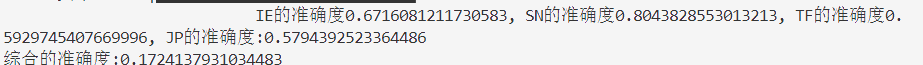
\includegraphics[width=0.618\textheight]{1}
		\title{KNN的实验结果}
	\end{figure}
	\subsection{结果分析}
	实验得到的KNN分类效果并不算好,可能和K的取值存在一定关系,但是KNN分类效果低于MLP在意料之中,MLP作为最简单的神经网络的泛化能力比MLP强倒也合理。
	\section{问题二}
	\subsection{解决的方法}
	为了解决这个问题,我采用了bert-base这一模型,同时借用transforms库和pytorch进行神经网络的搭建和训练,使用深度学习来解决这个文本分类问题。
	
	模型大致为Bert层->dropout层->线性层->ReLU层。
	
	选择这个模型的原因有:
	\begin{enumerate}
		\item BertBase模型的效果较好,而且参数量不算特别大(但也很大),利用BertBase可以提取文本特征,便于线性分类器分类。
		\item BertBase的使用更多,预训练过程中出现的问题更容易被解决。
	\end{enumerate}
	\subsection{进行的思考}
	部分同样的问题在上一章节已经讨论了,以下内容只讨论新的问题。
	\subsubsection{多句话文本要怎么进行处理}
	Bert模型其实理论上可以接受很长的文本,但是文本长度过长也会出现问题,经过统计,训练集中过长文本数量也不多,所以首先我们卡在Bert模型最大常规接受的长度512上。其次,我们的训练集其实是由很多句话组成的一个样本,那么我们是否应该对这个事情进行处理呢?我认为我们应该保证多句话还在同一个人的输入中,但是我们需要对训练集中使用的|||分隔符作出处理,处理时需要考虑这个分隔符应该直接换成句号吗?我思考后认为,不需要,应该直接换成Bert模型接受的[SEP]符号,表示一句话的结束。
	\subsection{实验结果}
	实验中最好的结果如下图:
	\begin{figure}[H]
		\centering
		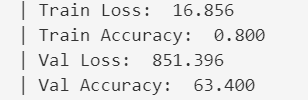
\includegraphics[width=0.618\textheight]{2}
		\caption{1轮训练中出现效果最好的测试结果}
	\end{figure}
	\subsection{结果分析}
	令人吃惊的是这个结果几乎已经达到了论文中出现的最好的结果,并且超过了课程群中给出的baseline,可能的原因是受限于设备性能,仅仅100个训练样本,1轮的训练也需要进行两到三个小时,导致训练样本的减少,却阴差阳错解决了类别不平衡的问题。因为神经网络的训练方法不同于KNN,类别不平衡问题不容易解决,神经网络可能会选择取巧来规避少样本数量的类别来获得更高的准确率。
	\section{问题三}
	经过实验,预训练模型的表现的的确确比传统机器学习方法要好。
	
	我认为可能的原因有以下几点:
	\begin{enumerate}
		\item \textbf{训练开销大:}这其实是在比较两种训练方法的参数量,前者KNN模型大小就是数据规模,后者经过调研BertBase的模型参数超过一亿个,通过上文提到的训练时长也可以显著看出来。
		
		\item \textbf{神经网络泛化能力强:}神经网络在自然语言处理方面的确具备天然的优势,层层特征的提取可以让模型几乎摸到了语义理解的核心内容,但是传统的机器学习方法,比如我使用的KNN,就仅仅只是进行相似度的匹配。
		
		\item \textbf{KNN没有使用提前特征提取:}这可能是深度学习方法完胜的一个重要原因,事实上我也尝试了进行特征提取,因为我试图用深度学习以外的方法与深度学习模型进行PK,所以我剩下的特征提取方法似乎只有PCA,但是就实际效果而言,PCA的使用过程也会导致训练时间的大大变长,所以这个想法被搁置,而神经网络本身就有特征提取的能力,在这一点上KNN吃了大亏。
		
		\item \textbf{预训练模型已经经过训练:}这一点其实再说明预训练模型已经经过了大量文本的洗礼,在数据量上比,KNN天然劣势,现在LLM的成功已经证明了,大量的数据并非毫无意义。
	\end{enumerate}
	虽然KNN表现不佳,但是我认为这不意味着传统机器学习方法的没落,KNN在时间开销上可以完胜深度学习算法,而且配合上PCA的使用,对数据进行处理,KNN效果也会得到提高,神经网络以一种范式化的训练就能够得到相当好的效果是建立在大量的数据和训练时间上,未必数据得到良好的处理的KNN就一定弱于神经网络,当然这只是在分类任务的范畴内,文本生成问题KNN可能就会束手无策,但是想要设计出能够比神经网络能力更强的KNN一定需要付出很多努力。
\end{document}	
